%%% template.tex
%%%
%%% This LaTeX source document can be used as the basis for your technical
%%% paper or abstract. Regardless of the length of your document, the commands
%%% are all the same.
%%% 
%%% The "\documentclass" command is the first command in your file. If you want to 
%%% prepare a version of your article with line numbers - a "review" version - 
%%% include the "review" parameter:
%%%    \documentclass[review]{acmsiggraph}
%%%

\documentclass{acmsiggraph}

%%% Title of your article or abstract.

\title{Running Minion:  Jump over Obstacles using Reinforcement Learning}

\author{
  Jiayu Li \\
  \texttt{lijiayu1027@ucla.edu}
  \and
  Zhaoyu Lu \\
  \texttt{zylu@ucla.edu}
  \and
  Siyuan Qi \\
  \texttt{syqi@cs.ucla.edu}
  \and
  Yutong Zhang \\
  \texttt{yzhang@cs.ucla.edu}
  }
\pdfauthor{Stephen N. Spencer}

%%% Used by the ``review'' variation; the online ID will be printed on 
%%% every page of the content.

% \TOGonlineid{45678}

% User-generated keywords.

\keywords{radiosity, global illumination, constant time}

% With the "\setcopyright" command the appropriate rights management text will be added
% to your document.

%\setcopyright{none}
%\setcopyright{acmcopyright}
%\setcopyright{acmlicensed}
\setcopyright{rightsretained}
%\setcopyright{usgov}
%\setcopyright{usgovmixed}
%\setcopyright{cagov}
%\setcopyright{cagovmixed}
%\setcopyright{rightsretained}

% The year of publication in the "\copyrightyear" command.

\copyrightyear{2016}

%%% Conference information, from the completed rights management form.
%%% The "\conferenceinfo" command has two parameters: 
%%%    - conference name
%%%    - conference date and location
%%% The "\isbn" field includes the year and month after the article ISBN.

\conferenceinfo{SIGGRAPH 2016 Posters}{July 24-28, 2016, Anaheim, CA} 
\isbn{978-1-4503-ABCD-E/16/07} 
\doi{http://doi.acm.org/10.1145/9999997.9999999}

\begin{document}

%%% This is the ``teaser'' command, which puts an figure, centered, below 
%%% the title and author information, and above the body of the content.


\maketitle

\begin{abstract}

In this project, we designed a virtural game where a Minion is running and jumping in order to survive in the harsh living environment. In the game setting, a Minion is controlled by our algorithm to run as far as possible. Along the way, the minion is running at a constant speed, and it needs to jump at an appropriate position to avoid collision with obstacles. We implemented the game in Pygame and used a reinforcement learning algorithm (Q-learning) to learn the learn a decision policy that guides the Minion to take actions at an appropriate timing. More specifically, we adopted the deep Q-learning network to train the Minion. The experiments results show the superiority of our work and the learned agent could manage to survive in the cruel living environment for a long time.

\end{abstract}

%% ------------------------------------- INTRODUCTION ------------------------------------- %%
\section{Introduction}
Recently, many people are fond of playing some causual games in their leisure time. Usually, these games will be very easy to learn and play, such as with only jump action in our game setting. Although the rule of  the game is simple, it is not easy to play the game by hand as the setting becomes much complicated and the obstacles generating more randomly. There has been many related works about self-palying games.  General Game Playing (GGP)\cite{genesereth2005general} was introduced to design game-playing systems with applicability to more than one specific game.P Spronck designed an adaptive game AI with dynamic scripting \cite{spronck2006adaptive}.

Learning game pattern for intelligent agent in a game can be a great challenge because it is difficult to figure out the relationship between high-dimenstional game input with game reward. A bunch of previous works apply machine learning algorithms to game policy learning. G.Chaslot, etc used Monte-Carlo Tree Search to implemente a frame work for game AI \cite{chaslot2008monte}. M Ponsen improved  adaptive game AI with evolutionary learning \cite{ponsen2004improving}. Despite these achievements, there have been some working using reinforcement learning to implement great game agents. M Bowling gave an An analysis
of stochastic game theory for multiagent reinforcement learning \cite{bowling2002multiagent} and deep Reinforcement learning proposed in \cite{mnih2013playing} gives the first convincing combination of deep neural network and reinforcement learning. It is able to learn policies for Atari 2600 games directly from high-dimenstional sensory input and create a competitve performace comparing to humans.  Arcade Learning Environment (ALE) \cite{bellemare13arcade} is a a platform and methodology for evaluating the development of general, domain-independent AI technology. ALE is a framework that designed to make it easy to develop self-play game agents and is also an experimental methodology that can be used to evaluate the performance of agents. 

In the following sections of this report, we will first briefly describe the learning methods we adapt in section4. Then the details of the game will be talked in section 5. Next, we would like to display our experiments and analyze the experimental results of our work. Finally, we will draw a conclusion and discuess about the possible future works.


%% ------------------------------------- RELATED WORK ------------------------------------- %%
\section{Related Work}
Reinforcement learning has been successfully applied to real-life environment for robotics controlling \cite{kober2013survey,abbeel2007helicopter}. To better cope with real-life situations, deep learning is a heated choice \cite{chen2014door}. Similarly, the researchers applied the algorithm to virtual environment and help the agents to finish tasks such as walking in the maze or chasing the pray \cite{manteghi2015maze,olsen2015co}. However, in those research in virtual setting, only linear function is used in reinforcement learning due to the chance of causing not convergence of the system. 

Previously, some researchers manage to combine deep learning and reinforcement learning \cite{mnih2013playing,gu02015monte}. [] develops an agent with Deep Q-learning (DQN) and make it learn to play video games in Atari 2600 emulator. They apply convolution neural network to store all Q values and the input to the network is only raw pixel of the game image. The experiment result is excellent and even outperform human-level control. The paper also applies experience-replace to break the dependency of sequential frame of the game procedure. The research is a good start to extent to more games. In this paper, DQN is adopted with Pygame environment \cite{tasfi2016PLE} in our experiment to make the agent learn to survive in new game environment.

%% ------------------------------------- MODEL ------------------------------------- %%
%\section{Model}


%% ------------------------------------- LEARNING ------------------------------------- %%
\section{Learning}
In this section, we briefly introduce the learning algorithm we adopted for this project. We first introduce the essential idea of Q-learning, and then introduce how to connect reinforcement learning to deep network.

\subsection{Q-learning}
In this project, we adopted a deep Q-learning network to train the agent. 
In traditional Q-learning, we consider tasks in which an agent interacts with an environment, in a sequence of actions, observations and rewards. Here the environment $\varepsilon$ is the game environment, in which at each time step the agent selects an action from a set of legitimate game actions $A = \{a_1, a_2, \cdots, a_k\}$. At each step $t$, the agent observes a game state $x_t$ and takes an action $a_t$, and then receives a reward $r_t$ which represents the change of the game score. The goal of the training algorithm is to let the agent interact with the environment in a way that maximizes the future rewards.

To better compute the total reward, the standard assumption of reinforcement learning is that the future rewards are discounted by a factor of $\gamma$ per time step. Hence the future accumulated return at time $t$ can be computed as $R_t = \sum_{t'=t}^T \gamma^{t'-t} r_{t'}$, where $T$ is the time when the game terminates.

Then the optimal action-value function $Q^{*}(s, a)$ is defined as the maximum expected return by choosing an optimal following strategy, after taking an action $a$ at state $s$:
$$
Q^{*}(s, a) = \max_{\pi} E[R_t | s_t = s, a_t = a, \pi]
$$
where $\pi$ is a policy of sequence-action mapping.

If we know the optimal value $Q^{s', a'}$ of the sequence $s'$ at the next time-step for all possible actions $a'$, then the optimal strategy is to select the action $a'$ maximizing the expected value of $r+\gamma Q^{*}(s', a')$:
$$
Q^{*}(s, a) = E[r + \gamma \max_{a'} Q^{*}(s', a') | s, a]
$$

it is common to use a function approximator to estimate the action-value function: $Q(s, a; \theta) \approx Q^{*}(s, a)$. It is typically a linear function approximator, but non-linear functions such as neural networks are also adopted to estimate the action-value function. A neural network function approximator with weights $\theta$ can be trained by minimizing a sequence of loss functions $L_i(\theta_i)$ that changes at each iteration $i$:
$$
L_i(\theta_i) = E_{s, a \sim \rho(s, a)} [(y_i - Q(s, a; \theta_i))^2]
$$
where $y_i = E[r + \gamma \max_{a'} Q(s', a' | \theta_{i-1}) | s, a] $ is the target for iteration $i$ and $\rho(s, a)$ is a probability distribution over sequences $s$ and actions $a$ that we refer to as the behaviour distribution. The parameters from the previous iteration $\theta_{i−1}$ are held fixed when optimising the loss function
$L_i(\theta_i)$.


\subsection{Deep Q-Learning Network}
We apply the deep Q-learning network to train our agent \cite{mnih2013playing}. Recent breakthroughs in computer vision and speech recognition have relied on efficiently training deep neural networks on very large training sets. The most successful approaches are trained directly from the raw inputs, using lightweight updates based on stochastic gradient descent. In this project, we use a reinforcement learning algorithm that takes the internal state as input.

The original architecture of connecting a neural network to reinforcement learning updates the parameters of a network that estimates the value function, directly from on-policy samples of experience, $s_t, a_t, r_t, s_{t+1}, a_{t+1}$, drawn from the algorithm’s interactions with the environment (or by self-play, in the case of backgammon). Recently, a new architecture exploiting the deep neural network and scalable RL algorithms was proposed. In this approach, a technique known as experience-replay is utilized. The agent's experiences $e_t={s_t, a_t, r_t, s_{t+1}}$ at each time step is stored in a dataset $D={e_1, \cdots, e_N}$. The experiences are pooled over many episodes into a replay memory. In the inner loop of the algorithm, the Q-learning updates are applied to samples of experience, $e \sim D$, drawn from the pool of stored samples (replay memory). After performing experience replay,
the agent selects and executes an action according to an $\epsilon$-greedy policy. Since using histories of arbitrary length as inputs to a neural network can be difficult, the Q-function instead works on fixed length representation of histories produced by a function $phi$. 

In practice, this algorithm only stores the last N experience tuples in the replay memory, and samples uniformly at random from D when performing updates. This approach is in some respects limited since the memory buffer does not differentiate important transitions and always overwrites with recent transitions due to the finite memory size N. Similarly, the uniform sampling gives equal importance to all transitions in the replay memory. 


%% ------------------------------------- EXPERIMENTS ------------------------------------- %%
\section{Experiments}
\subsection{Game Environment} 
This project(game) is implemented by Pygame, a cross-platfom set of Python modules designed for creating games. By using Pygame, we can easily build up a game scenery for our intelligent agent to play with. Furthermore, Python has many open-source machine learning packages. Therefore we can simply focus on training our agent to run and jump through all the obstacles instead of spending much time on writing common learning algorithm from scratch. These set of modules allow us to write fully featured games and multimedia programs with small amount of code. It is very easy to use and truly portable. PyGame Learning Environment (PLE) is the learning environment we used in this work. PLE mimicks the Arcade Learning Environment \cite{bellemare13arcade} interface, allowing a quick start to reinforcement learning in python. The goal of PLE is allow practitioners to focus design of models and experiments instead of environment design. Through PLE, we can implement the whole learning agent without major modification of the game.

\subsubsection{Graphics(User interface)}
The Minion has three image status when running. We set these three status chaning repeatedly with certain pattern. When jumping, the Minion has another image status. The obstacle we used here is a pipe shown in figure \ref{fig:minion}.


\begin{figure}[ht]
  \centering
  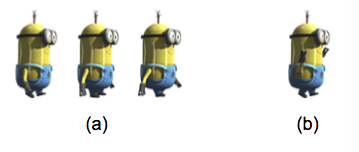
\includegraphics[width=3.0in]{../fig/minion.png}
  \caption{(a) Three patterns of the running minion. (b) Image of a jumping minion.}
  \label{fig:minion}
\end{figure}


\begin{figure}[ht]
  \centering
  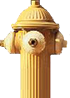
\includegraphics[width=50pt]{../fig/obstacle.png}
  \caption{Obstacles in the game.}
  \label{fig:obstacle}
\end{figure}


\begin{figure}[ht]
  \centering
  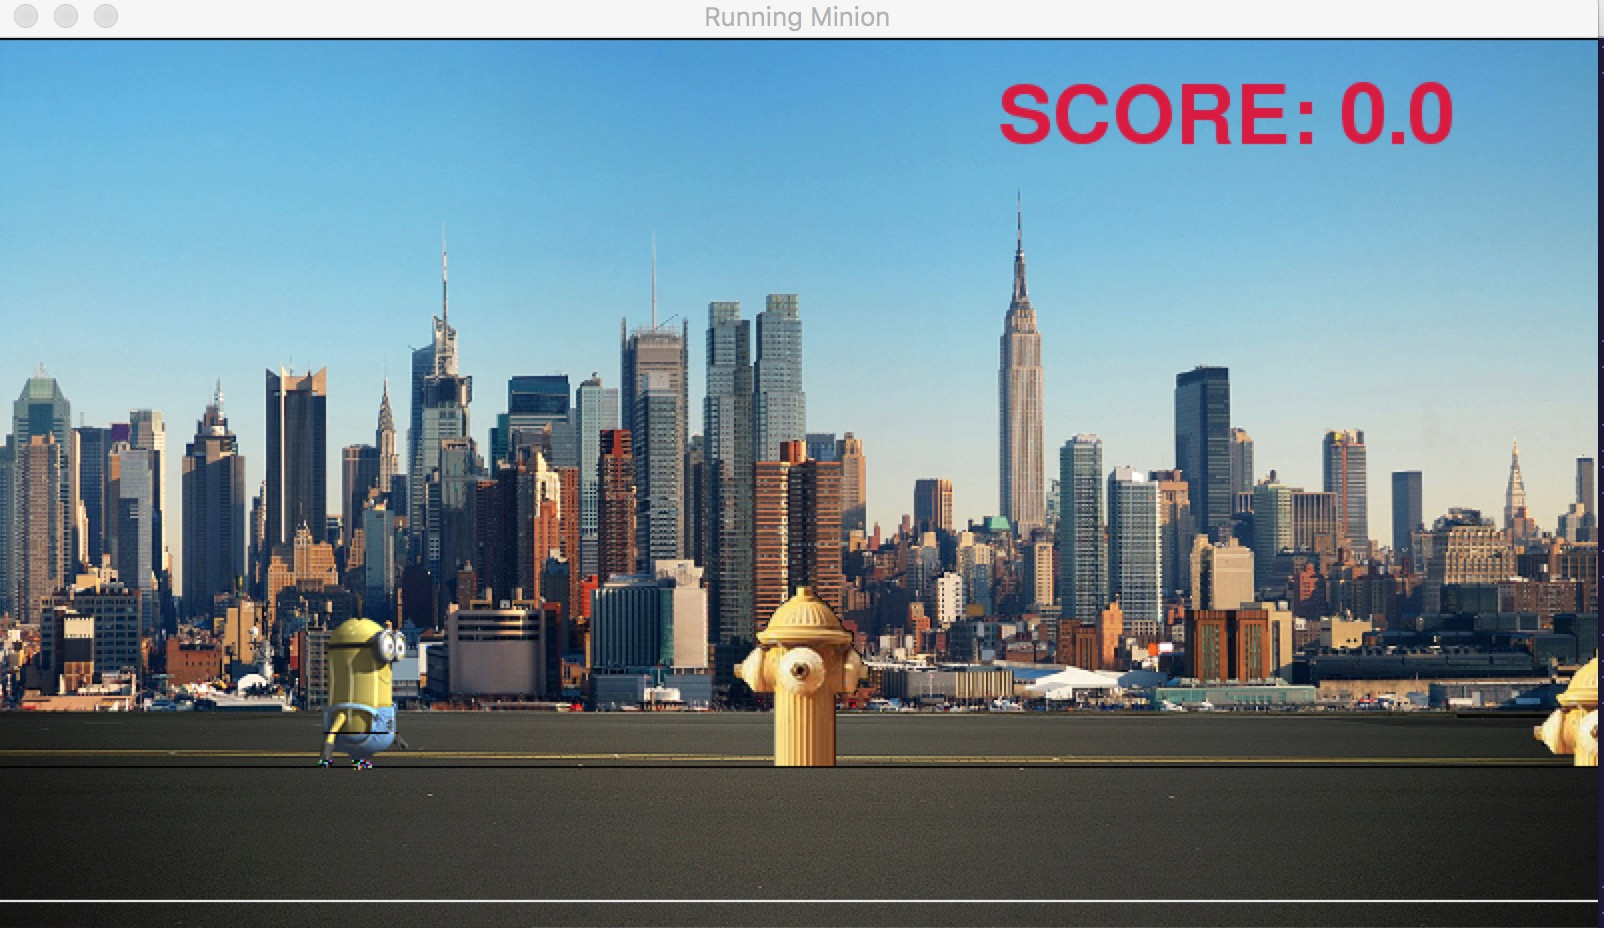
\includegraphics[width=3.0in]{../fig/interface.jpg}
  \caption{The game interface.}
  \label{fig:interface}
\end{figure}

\subsubsection{Game setting}
(1) Input parameters
For every step in the game process, we keep track of three game states: Horizontal distance between obstacle and agent, Height of obstacle and life status of the agent.
(2) Actions
For every step, the agent can choose to take an action and jump or do nothing.
(3) Rewards
In our game setting, if the Minion passes through one obstacle, it will gain 1 reward but will lose 5 rewards if hit on the pipe. Besides, in order to combine the appropriate rate of jumping, we set a penalty to the score whenever the Minion jump, which means the agent will lose 0.2 every time it jumps. 

After one game, the more rewards the agent gained, the better model we have learned.

\subsubsection{Game Learning Procedure}

Step 1: Observe what state the Minion is in and perform the action (jump or not jump) that maximizes expected reward. Let the game engine perform its “tick”. Now the Minion is in a next state s’.
Step 2: Observe the new state s’, and the reward associated with it.
Step 3: Update the Q array according to the Q-Learning rule and pass the array to the learning procedure.


\subsubsection{Experiment results}
(1) Stability (Image)
In reinforcement learning, the evaluation of an agent is difficult to compute during training. Instead, we compute the total reward the agent collects in one episode. From the figure, we can find that the average total reward is very noisy. This is because a small change to the weight of stragety will largely change the state of policy and thus greatly affect the reward of that policy. 

(2) Different reward strategies for agent learning





\begin{figure}[ht]
  \centering
  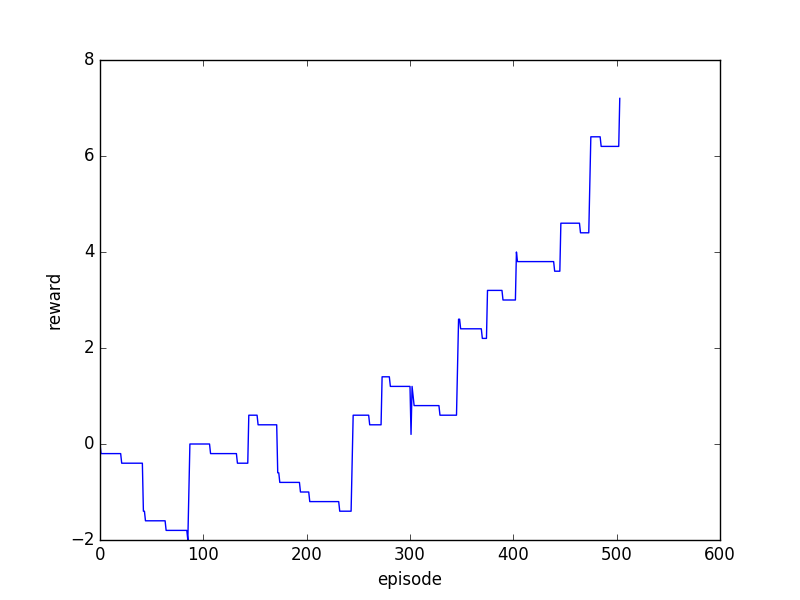
\includegraphics[width=3.0in]{../fig/reward_in_testing_5000.png}
  \caption{Testing result.''}
  \label{fig:result}
\end{figure}


%% ------------------------------------- CONCLUSION ------------------------------------- %%
\section{Conclusion \& Future Work}
In this project, we created a game where a Minion is running and supposed to jump at certain position to avoid hitting the obstacles. We used Q-Learning to train the Minion agent and achieved Minion-self-play. The experiments results displayed demonstrate that this learned agent can evolve and gain better performance through generation. 
For future work, we would like to modifify the game and create a much more realistic 3D game with complex settings. What is more, we can add more forms of obstacles (gaps, different shapes of obstalces, etc) in the future to increase the difficulity level of the game. Or even we can try more learning algorithms (NEAT) and do some compasiron with Q-learning.


\section*{Acknowledgements}

To Robert, for all the bagels.

\bibliographystyle{acmsiggraph}
\nocite{*}
\bibliography{report}
\end{document}
